\documentclass{article}  
\usepackage{graphicx}
\usepackage[utf8]{inputenc}
\usepackage[T1]{fontenc}
\usepackage{float}
\usepackage[italian]{babel}
\usepackage{listings}
\usepackage[usenames]{color}
\usepackage{natbib}
\usepackage{siunitx}
\usepackage[strict]{changepage}
\usepackage{physics}
\usepackage{wrapfig}
\usepackage[a4paper, top=2cm, bottom=2cm, right=2cm, left=2cm]{geometry}
\usepackage{array}
\usepackage{color}
\usepackage{colortbl}
\usepackage{amsmath}
\usepackage{amssymb}
\usepackage{multirow}
\usepackage{enumitem}
\usepackage{hyperref}
\usepackage{times}
\usepackage{booktabs}



\title{Relazione di laboratorio: studio di catena elettronica}
\author{Docente: dott. Garfagnini, dott. Lunardon \\
Gruppo 14}
\date{Anno accademico 2019/20}

\begin{document}



\maketitle

\begin{itemize}
    \item[$\circ$] Aidin Attar - 1170698 - aidin.attar@studenti.unipd.it
    \item[$\circ$] Ema Baci - 1171107 – ema.baci@studenti.unipd.it
    \item[$\circ$] Alessandro Bianchetti – 1162147 – alessandro.bianchetti@studenti.unipd.it
\end{itemize}

\vspace{3 cm}
\begin{large}\textsc{\textbf{Scopo dell'esperienza}: studio della curva di trasferimento di un amplificatore invertente, del circuito con amplificatore delle differenze (non invertente), dei circuiti sommatore invertente, derivatore, raddrizzatore di precisione.} 
\end{large}
\vspace{8.5cm}

\begin{figure}[H]
\centering

\includegraphics[scale=0.5, angle=0]{unipd_logo.png}
\end{figure}

%\newpage \tableofcontents \newpage

\twocolumn

\subsection*{Descrizione dell'apparato} La seguente esperienza è stata svolta sul banco di lavoro 1. L'apparato di misura consiste di 
un oscilloscopio digitale Tektronix TBS 1102B EDU, un generatore di funzioni Tektronix AFG 1022, un alimentatore di tensione continua stabilizzato,
due multimetri digitali (metrix e ) e una scheda Arduino Due. 
Si è inoltre fatto uso di due integrati TL082C contenenti in tutto 4 amplificatori operazionali.

I circuiti studiati sono stati costruiti sulla basetta millefori alimentando gli amplificatori operazionali come nello schema riportato 
in figura \ref{fig:alimentazione}, in particolare si è fatto uso del modello TL082 JFET; dopodiché si sono 
costruiti i circuiti da studiare;  i valori misurati di resistenze e capacità utilizzate verranno riportati in seguito.
Si è inoltre fatto uso di due sonde con fattore di attenuazione 10x precedentemente compensate per la visualizzazione del 
segnale nei due canali dell'oscilloscopio.

Per l'analisi dati sono stati utilizzati programmi scritti in c++, root, gnuplot ed Excel.

\begin{center}
\begin{figure}[H]
\centering
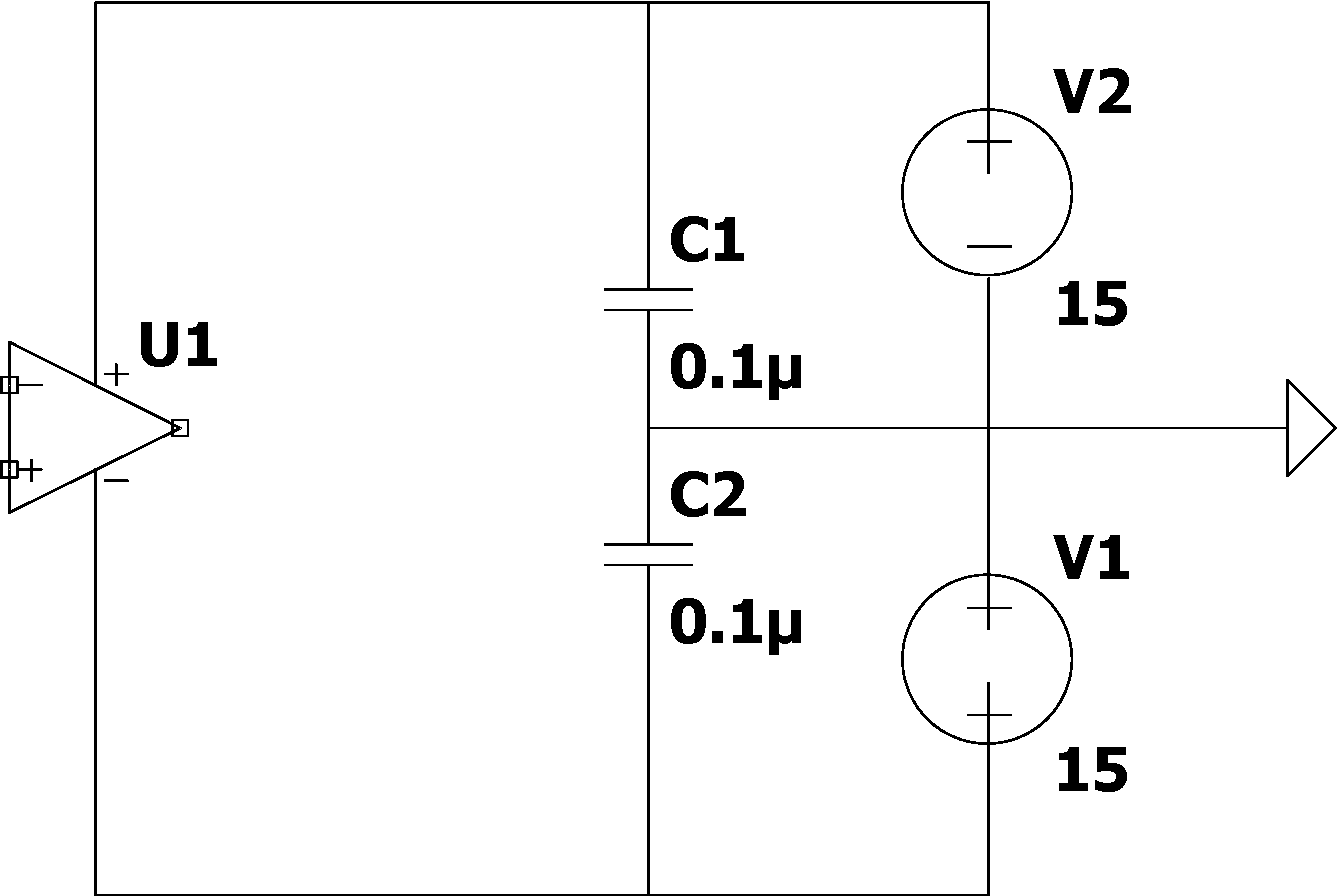
\includegraphics[scale=0.1875, angle=0]{alimentazione.pdf}
\caption{ Schema per l'alimentazione dell'operazionale }
\label{fig:alimentazione}
\end{figure}
\end{center} 

\section{Preamplificatore di carica}

\subsection{Breve discussione del circuito}

Lo scopo dell'esperienza completa è costruire un circuito che possa rilevare piccoli segnali, amplificarli tanto da poterli processare con più facilità
e poi amplificarli ulteriormente per offrirli allo sperimentatore. Il primo passo della realizzazione di tale \textit{catena elettronica} è il circuito
preamplificatore. Qui il generatore di funzione è utilizzato proprio per simulare piccoli segnali di cui sopra analoghi a quelli che proverrebbero tipicamente 
da esperienze di spettrocopia: si forniscono dunque in ingresso impulsi di tensione (PULSE) come quelli che produrrebbe il passaggio di una radiazione ionizzante in 
un volume di gas. 
Si è dunque costruito il circuito come in figura

\begin{center}
\begin{figure}[H]
\centering
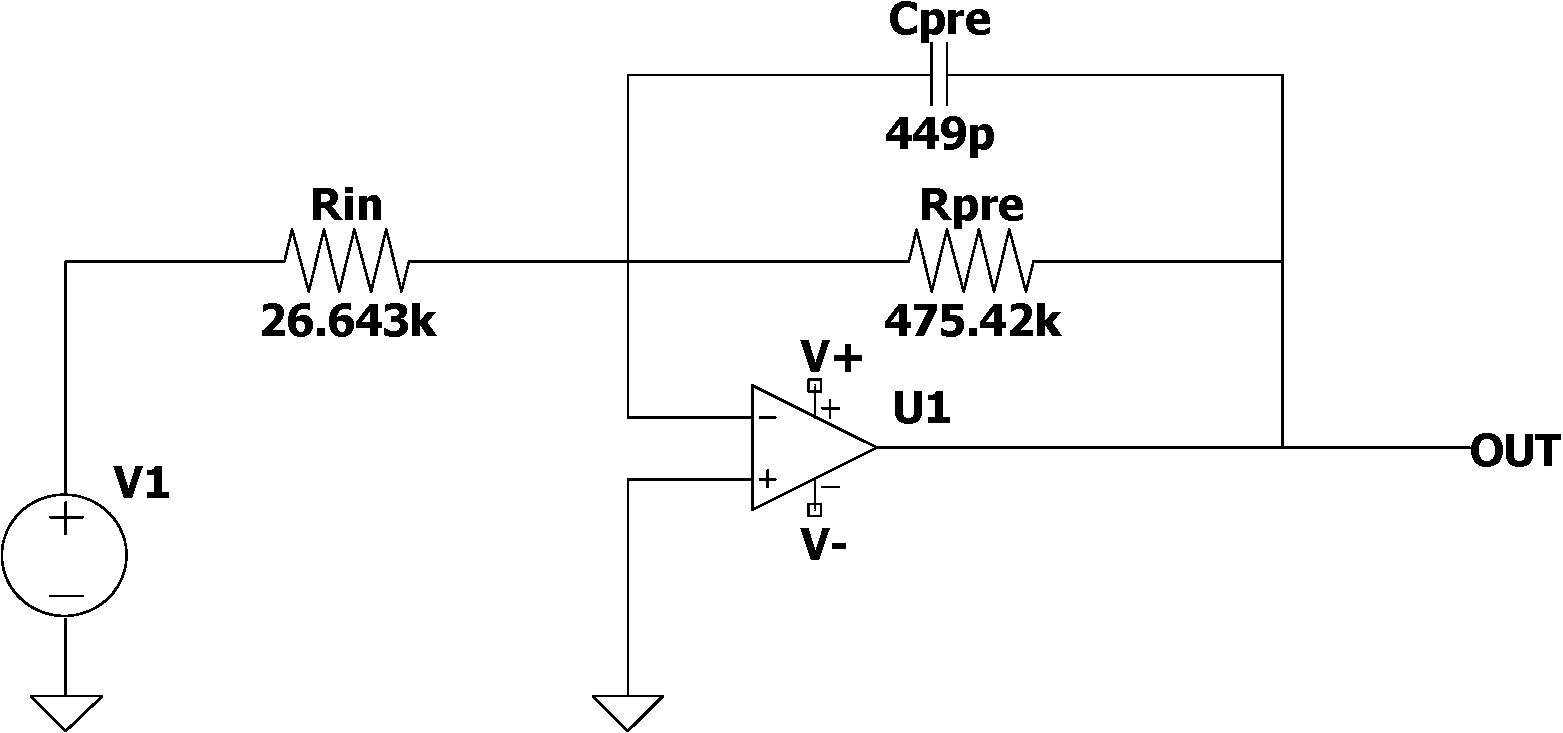
\includegraphics[scale=0.1875, angle=0]{preamp.pdf}
\caption{ Circuito amplificatore di carica }
\label{fig:preamp}
\end{figure}
\end{center}

la cui funzione di trasferimento è data, nel formalismo di Laplace, da

\begin{equation}
    \label{eqn:preamp_Laplace}
    H(s) = -\frac{R_{pre}}{R_{in}} \frac{1}{1+sR_{pre}C_{pre}}
\end{equation}

in cui possiamo effettuare la sostituzione $s \longleftrightarrow i\omega$ per riprodurre la soluzione stazionaria. Considerando poi
solamente il modulo, e definendo il tempo caratteristico $\tau_{pre}=R_{pre}C_{pre}$, avremo

\begin{equation}
    \label{eqn:preamp_trasf}
    H(\omega) = \frac{R_{pre}}{R_{in}} \frac{1}{\sqrt{1+\omega^2\tau_{pre}^2}}
\end{equation}

Si osserva inoltre che inserendo nella formula \ref{eqn:preamp_Laplace} la trasformata di Laplace dell'impulso di tensione, pari a 
$V_{in}$/s, si otterrà in uscita, antitrasformando opportunamente, un segnale esponenziale corrispondente a

\begin{equation}
    \label{eqn:Vout1_preamp}
    V_{pre}^{pulse}(t) = -\frac{R_{pre}}{R_{in}}V_{in}(1-e^{-\frac{t}{\tau_{pre}}})
\end{equation}

Quest'ultima è valida finché dura l'impulso di tensione: essendo $T_{pulse} << \tau_{pre}$, potremo considerare l'espansione in 
serie di Taylor della \ref{eqn:Vout1_preamp}, ottenendo una discesa lineare. Tale discesa lineare si interromperà all'esaurirsi dell'
impulso in ingresso, lasciando posto alla formula della scarica del condensatore $C_{pre}$, caricato proprio dallo stesso impulso.
Ne risulta un grafico che ha un picco negativo $V_{pre}^{max}$ in corrispondenza di t = $T_{pulse}$, per poi risalire con la curva esponenziale
dettata da

\begin{equation}
    \label{eqn:Vout2_preamp}
    V_{pre}^{RC}(t) = V_{pre}^{max}e^{-\frac{t}{\tau_{pre}}}.
\end{equation}

Si precisa che sono stati suggeriti dei valori per i parametri del circuito $\tau_{pre,th} = 220 \mu s$ e $C_{pre} = 450 pF$, con $R_{pre}$ calcolato di 
conseguenza. Pertanto i valori misurati con il multimetro sono

\[R_{pre} = (475.4 \pm 0.2)k\Omega \quad \sigma_{\%}=0.04 \%\]
\[C_{pre} = (149 \pm 14) pF \quad \sigma_{\%}=3.1 \%\]
\[\tau_{pre,th} = (213 \pm 7)\mu s \quad \sigma_{\%}=3.1 \%\]

\subsection{Discussione dati}

Si è successivamente impostato un impulso della durata di $T_{pulse}$ = $2 \mu s$: sapendo inoltre che la carica da iniettare 
corrispondeva a $Q_{in}^{th}$ = $80 pC$ e che la resistenza di ingresso scelta misurava $R_{in}=(26.64\pm0.01) k\Omega$ ($\sigma_{\%}=0.04\%$), 
si è selezionata l'altezza $V_{in}$ dell'impulso in modo che fosse soddisfatta la relazione

\begin{equation}
    \label{eqn:Qin}
    Q_{in} = \frac{V_{in}}{R_{in}} T_{pulse}.
\end{equation}

Ne si è ricavato $V_{in}^{th}$ =1.06 V. Per controllare la correttezza del circuito si è misurato il picco $V_{pre}^{max}$, che sarà
dato, utilizzando l'approssimazione della \ref{eqn:Vout1_preamp}, da

\begin{equation}
    \label{eqn:Vpre_max}
    V_{pre}^{max} = -\frac{R_{pre}}{R_{in}} V_{in} \frac{T_{pulse}}{\tau_{pre}} = - \frac{Q_{in}}{C_{pre}}
\end{equation}

da cui, inserendo il valore misurato $V_{in}^{th}=(1.02\pm 0.02) V$, si ricava $V_{pre,th}^{max} =  (-170 \pm 6) mV$. Invece dalla 
misura si ottiene $V_{pre,sper}^{max} = (-176 \pm 4) mV$, per cui $\lambda = 0.76$ e lo scostamento percentuale è $\epsilon = 3.2 \%$, 
ossia il valore misurato è ottimamente compatibile con quello atteso.

Si è inoltre la verificata la linearità tra $Q_{in}$ e $V_{pre}^{max}$ descritta da \ref{eqn:Vpre_max} variando la durata dell'impulso
in ingresso e quindi la carica iniettata nel circuito secondo \ref{eqn:Qin}. Si riportano quindi in grafico i punti, la retta 
interpolante e i principali parametri di bontà del fit. 

\begin{center}
\begin{figure}[H]
\centering
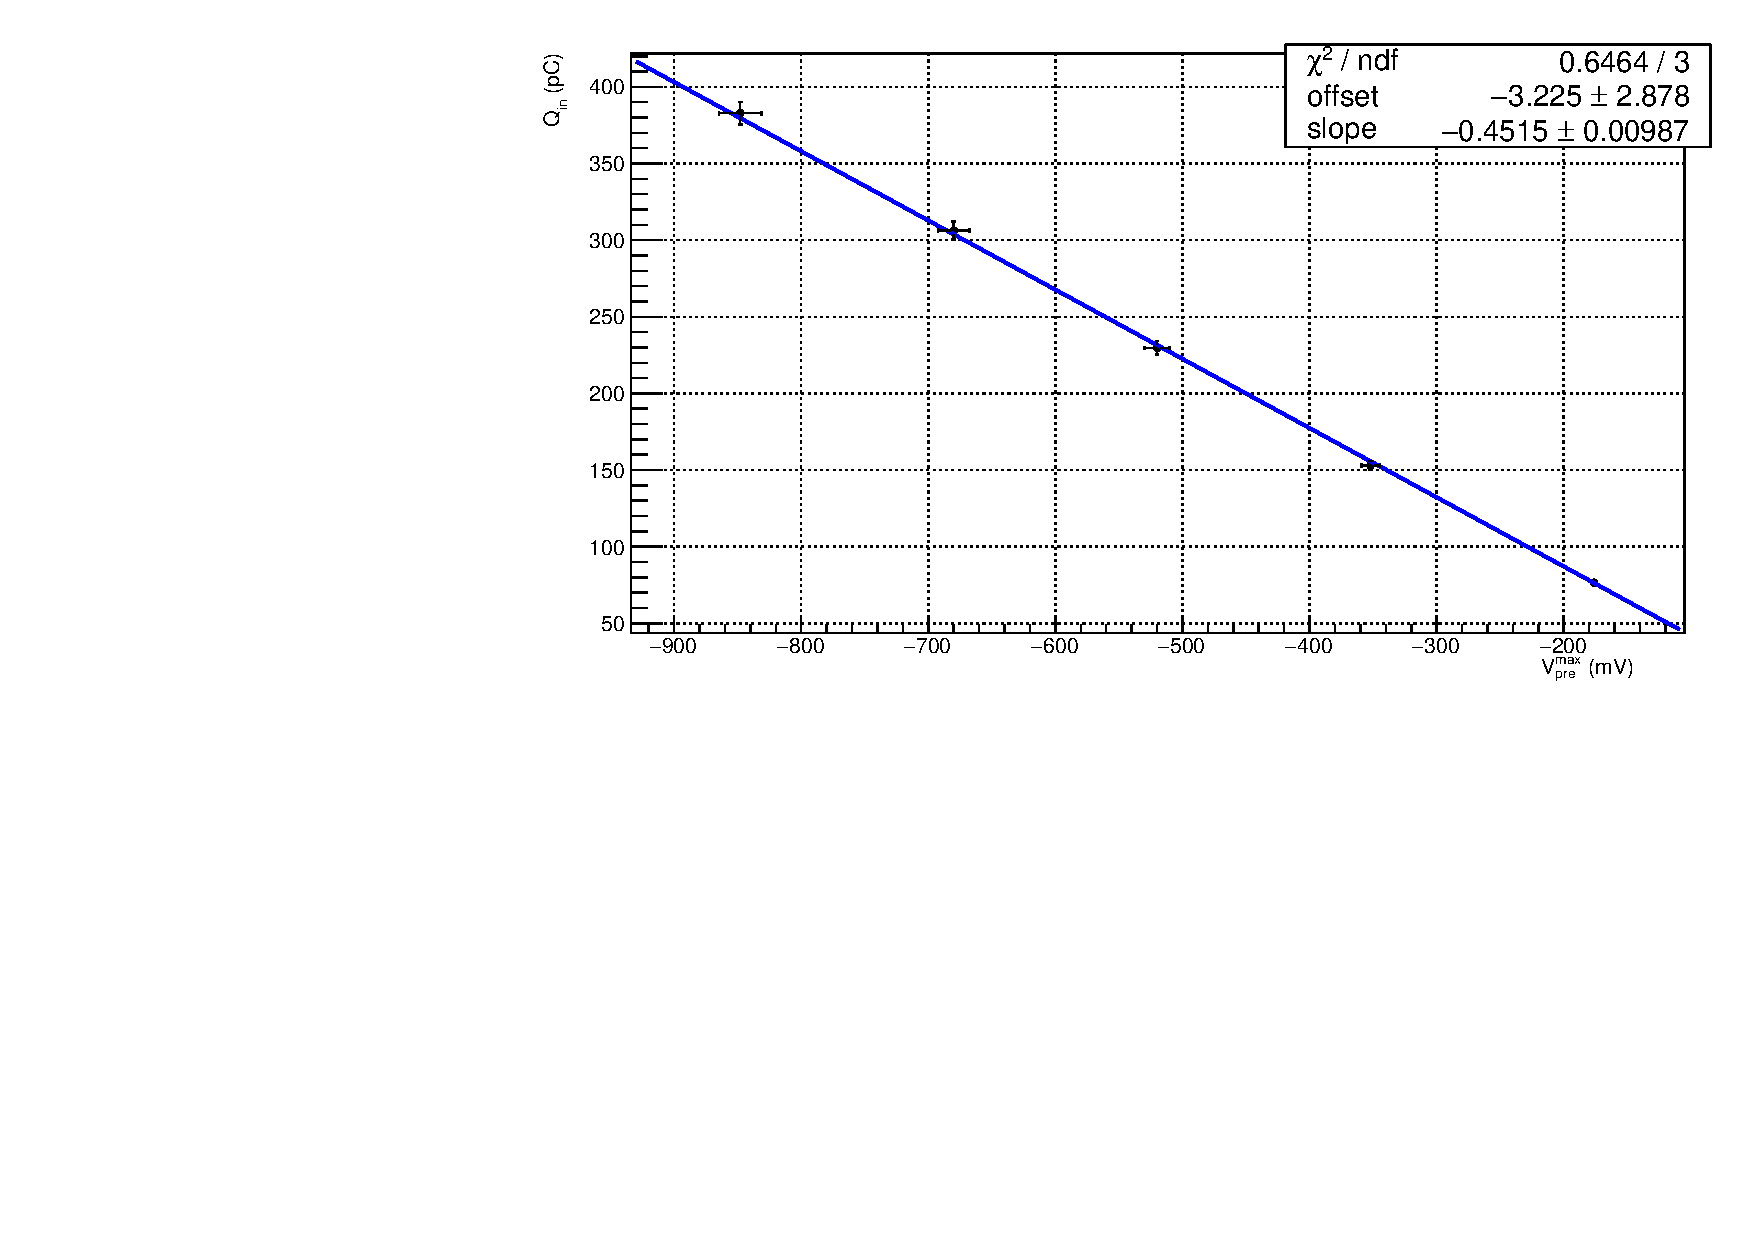
\includegraphics[scale=0.4, angle=0]{fitpreamp.pdf}
\caption{ Carica iniettata e picco di tensione in uscita}
\label{fig:QinvsVpre}
\end{figure}
\end{center}

\begin{center}
\begin{figure}[H]
\centering
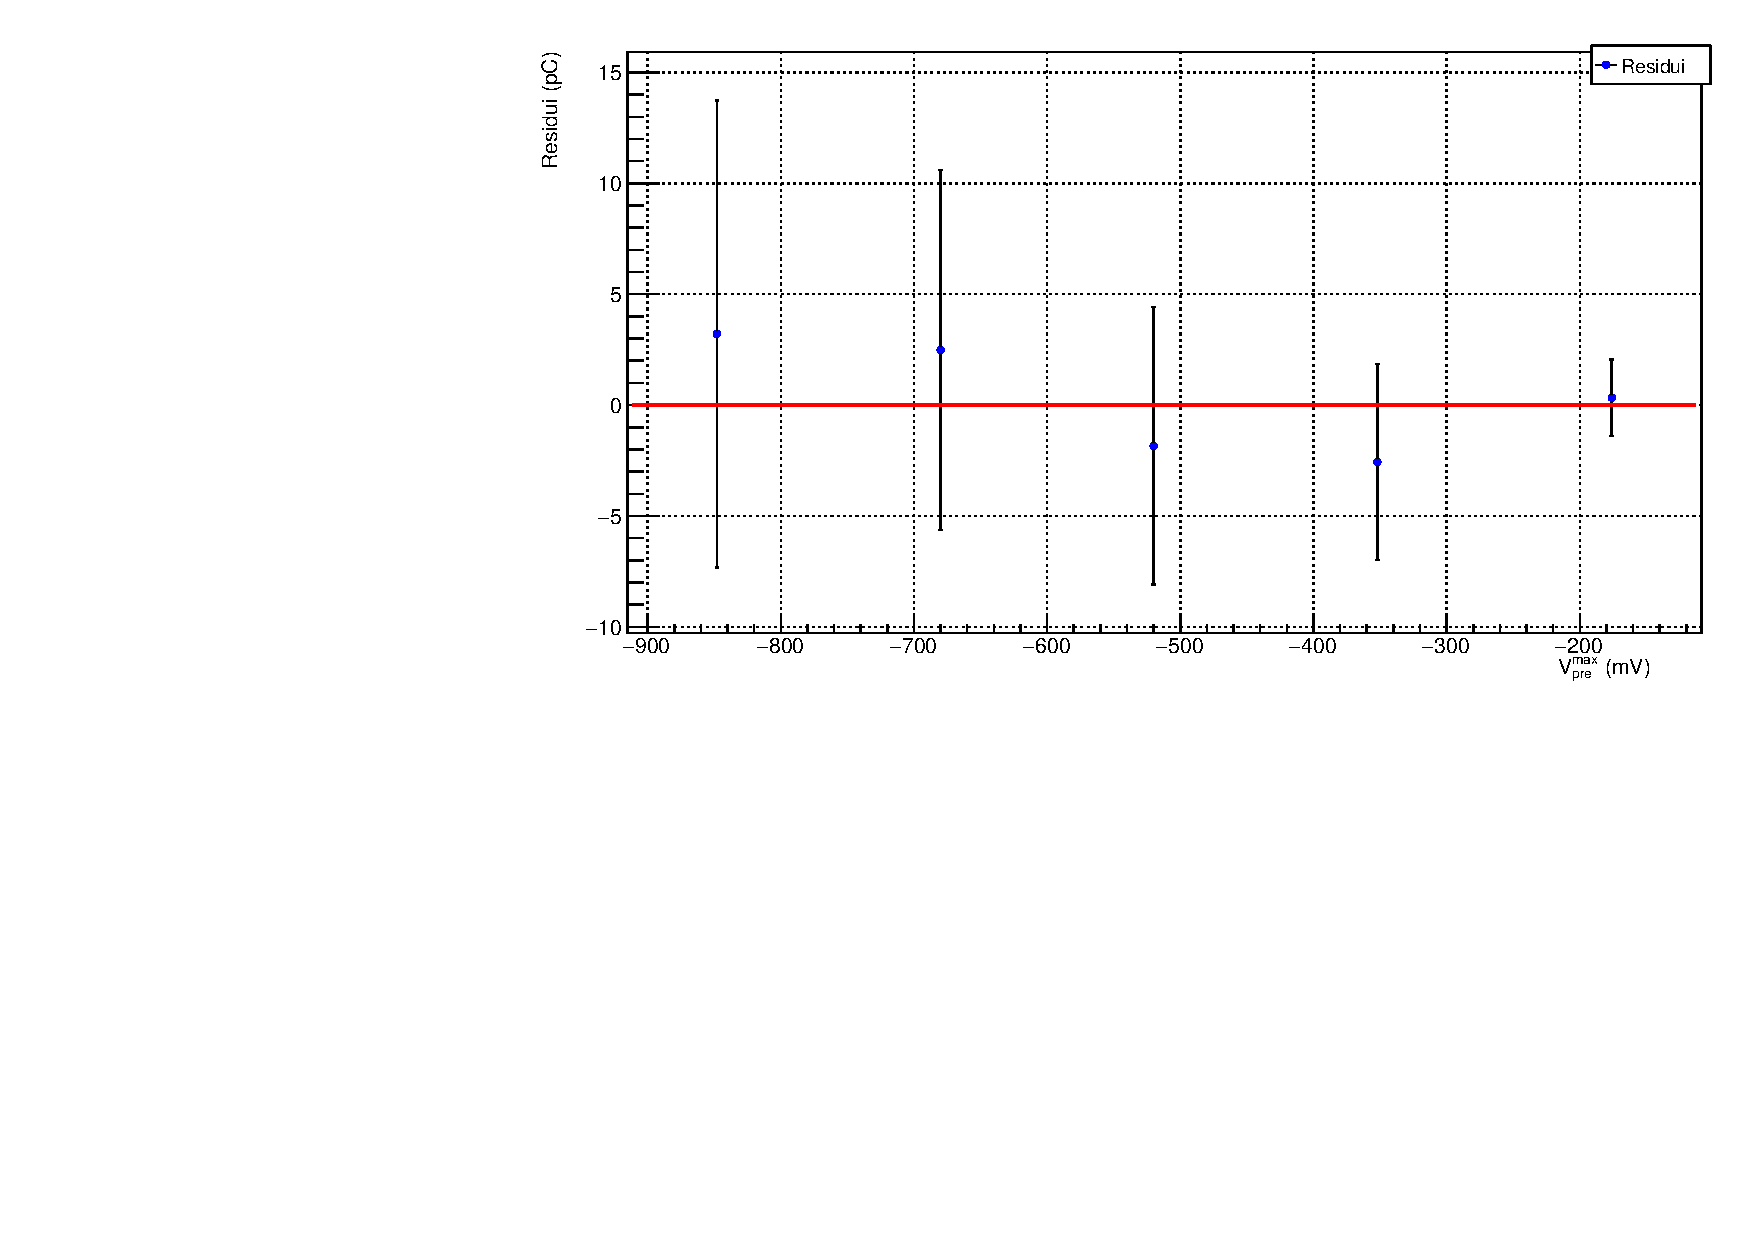
\includegraphics[scale=0.4, angle=0]{residuipreamp.pdf}
\caption{Grafico dei residui della relazione tra $Q_{in}$ e $V_{pre}^{max}$}
\label{fig:QinvsVpre_res}
\end{figure}
\end{center}

\begin{table}[ht]
    \centering
    \begin{tabular}{ccccc}
        \toprule
        $\sigma_{y, post}$    &$\chi^{(2)}$    &$\lambda_{\chi}$   &$\rho$ &t   \\
        \midrule
        0.05 V                &0.65            &0.96               &-0.9998&-63\\
        \bottomrule
    \end{tabular}
    \caption{parametri di verifica della bontà del fit}
\end{table}

Gli estimatori danno tutti risposta positiva, quindi possiamo concludere che la relaizone lineare è ben verificata.
Inoltre dal valore di pendenza, considerando la legge lineare \ref{eqn:Vpre_max}, è possibile ottenere una stima sperimentale della capacità $C_{pre}$, 
da confrontare con il valore misurato. Si ricava quindi $C_{pre,sper} = (452\pm 10)pF$, che ha $\lambda = 0.15 $ rispetto al valore misurato.

Inoltre dallo studio della \ref{eqn:Vout2_preamp}, e in particolare della sua linearizzazione logaritmica, è possibile ricavare
una stima sperimentale di $\tau_{pre}$. Infatti applicando il logaritmo naturale ottengo

\begin{equation}
    \log V(t) = \log V_{pre}^{max} - \frac{t}{\tau_{pre}}
\end{equation}

per cui si trova una relazione lineare tra $\log V(t)$ e t, da cui $\tau_{pre}$=-1/b con b slope del fit.
Si riporta il grafico di tempi e lograitmi delle tensioni, interpolati linearmente, e il relativo grafico dei residui

\begin{center}
\begin{figure}[H]
\centering
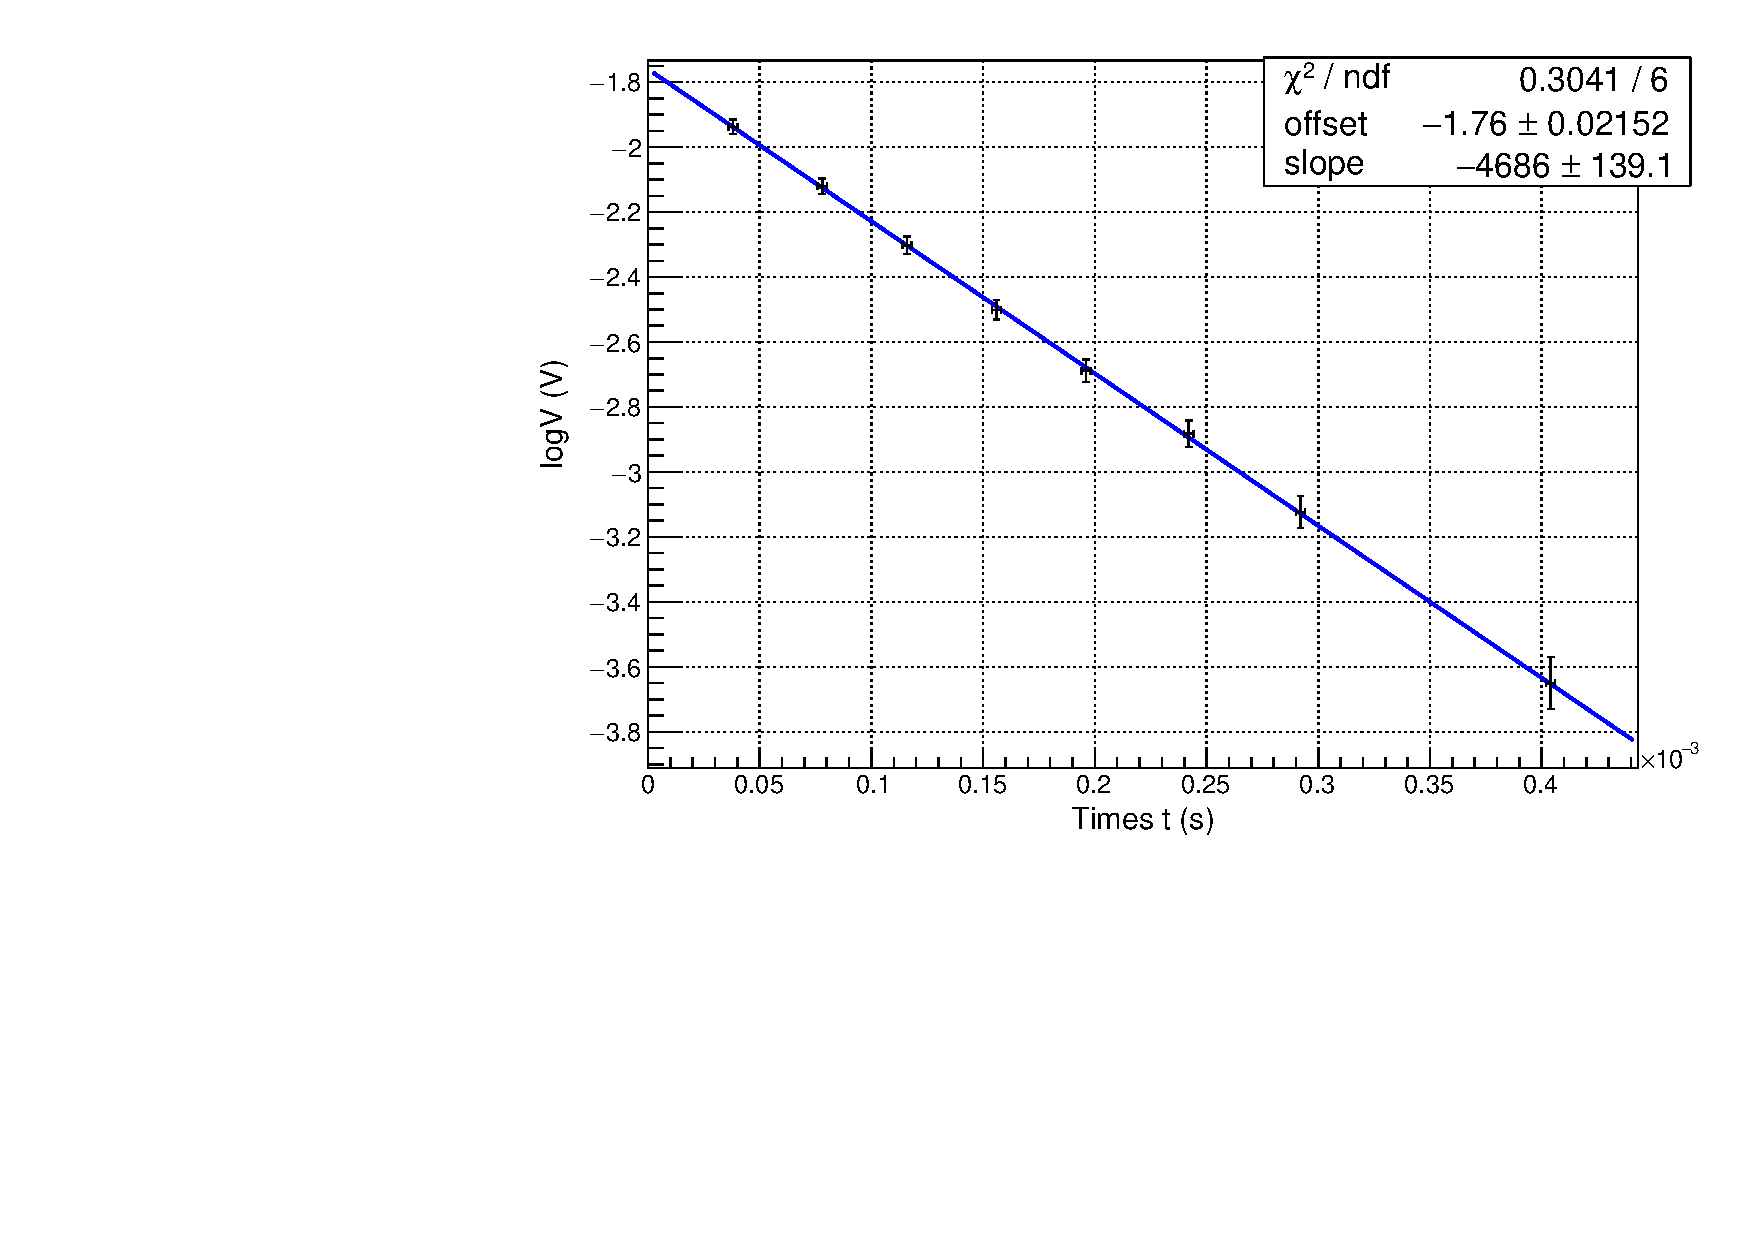
\includegraphics[scale=0.4, angle=0]{preampRC.pdf}
\caption{Relazione lineare tra logaritmi delle tensioni e tempi}
\label{fig:QinvsVpre}
\end{figure}
\end{center}

\begin{center}
\begin{figure}[H]
\centering
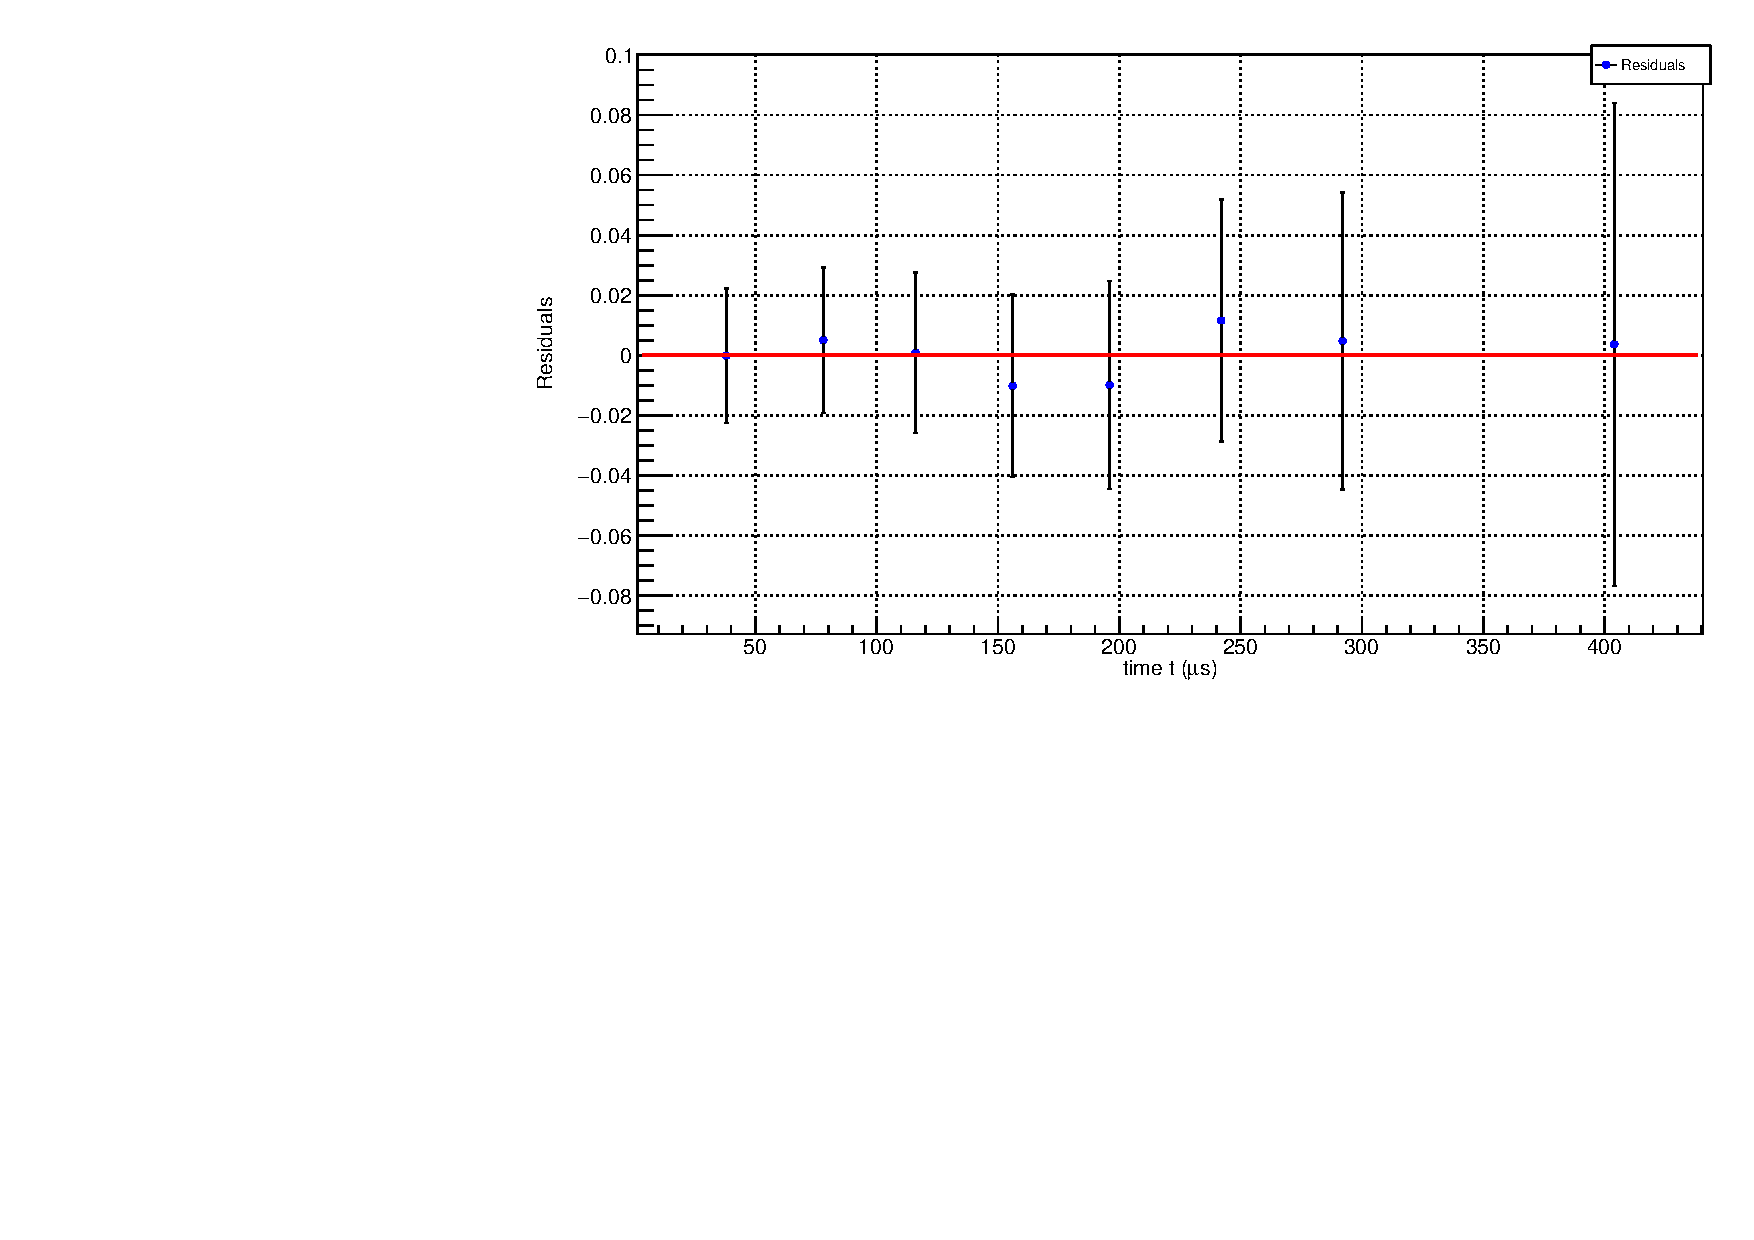
\includegraphics[scale=0.4, angle=0]{preampRCresidui.pdf}
\caption{Grafico dei residui della relazione tra $\log V$ e t}
\label{fig:QinvsVpre}
\end{figure}
\end{center}

\begin{table}[ht]
    \centering
    \begin{tabular}{ccccc}
        \toprule
        $\sigma_{y, post}$    &$\chi^{(2)}$    &$\lambda_{\chi}$   &$\rho$ &t   \\
        \midrule
        0.05 V                &3.36            &1.33               &-0.9998&-154\\
        \bottomrule
    \end{tabular}
    \caption{parametri di verifica della bontà del fit}
\end{table}

Dal valore della pendenza, come anticipato prima, ricaviamo una stima di $\tau_{pre,sper}$. A scopo di controllo, è inoltre possibile 
ottenere una valutazione di $V_{pre}^{max}$ usando il parametro di offset a sapendo $V_{pre}^{max} = e^a$. Si riportano quindi i due
valori calcolati con i loro errori calcolati per propagazione.

\[\tau_{pre,sper} = (213 \pm 6)\mu s \quad \sigma_{\%} = 2.9 \%\]
\[V_{pre}^{max} = (-172 \pm 3)mV \quad \sigma_{\%} = 2.0 \%\]

che risultano ottimamente compatibili con i valori attesi $V:{pre.th}^{max}$ e $\tau_{pre,th}$, in quanto $\lambda_{\tau} = 0.01$
e $\lambda_{V}=0.2$.

Si è infine effettuato uno studio in frequenza del circuito con lo scopo di verificare la \ref{eqn:preamp_trasf}, variando la frequenza
e verificando il variare del modulo dell'ampiezza di fronte a un ingresso sinusoidale.
Si riporta in particolare il grafico di Bode che raffigura frequenza e amplificazione in dB: ai punti sperimentali si è affiancata
anche la simulazione effettuata su LTspice e il modello teorico rappresentato dalla \ref{eqn:preamp_trasf}.

\begin{center}
\begin{figure}[H]
\centering
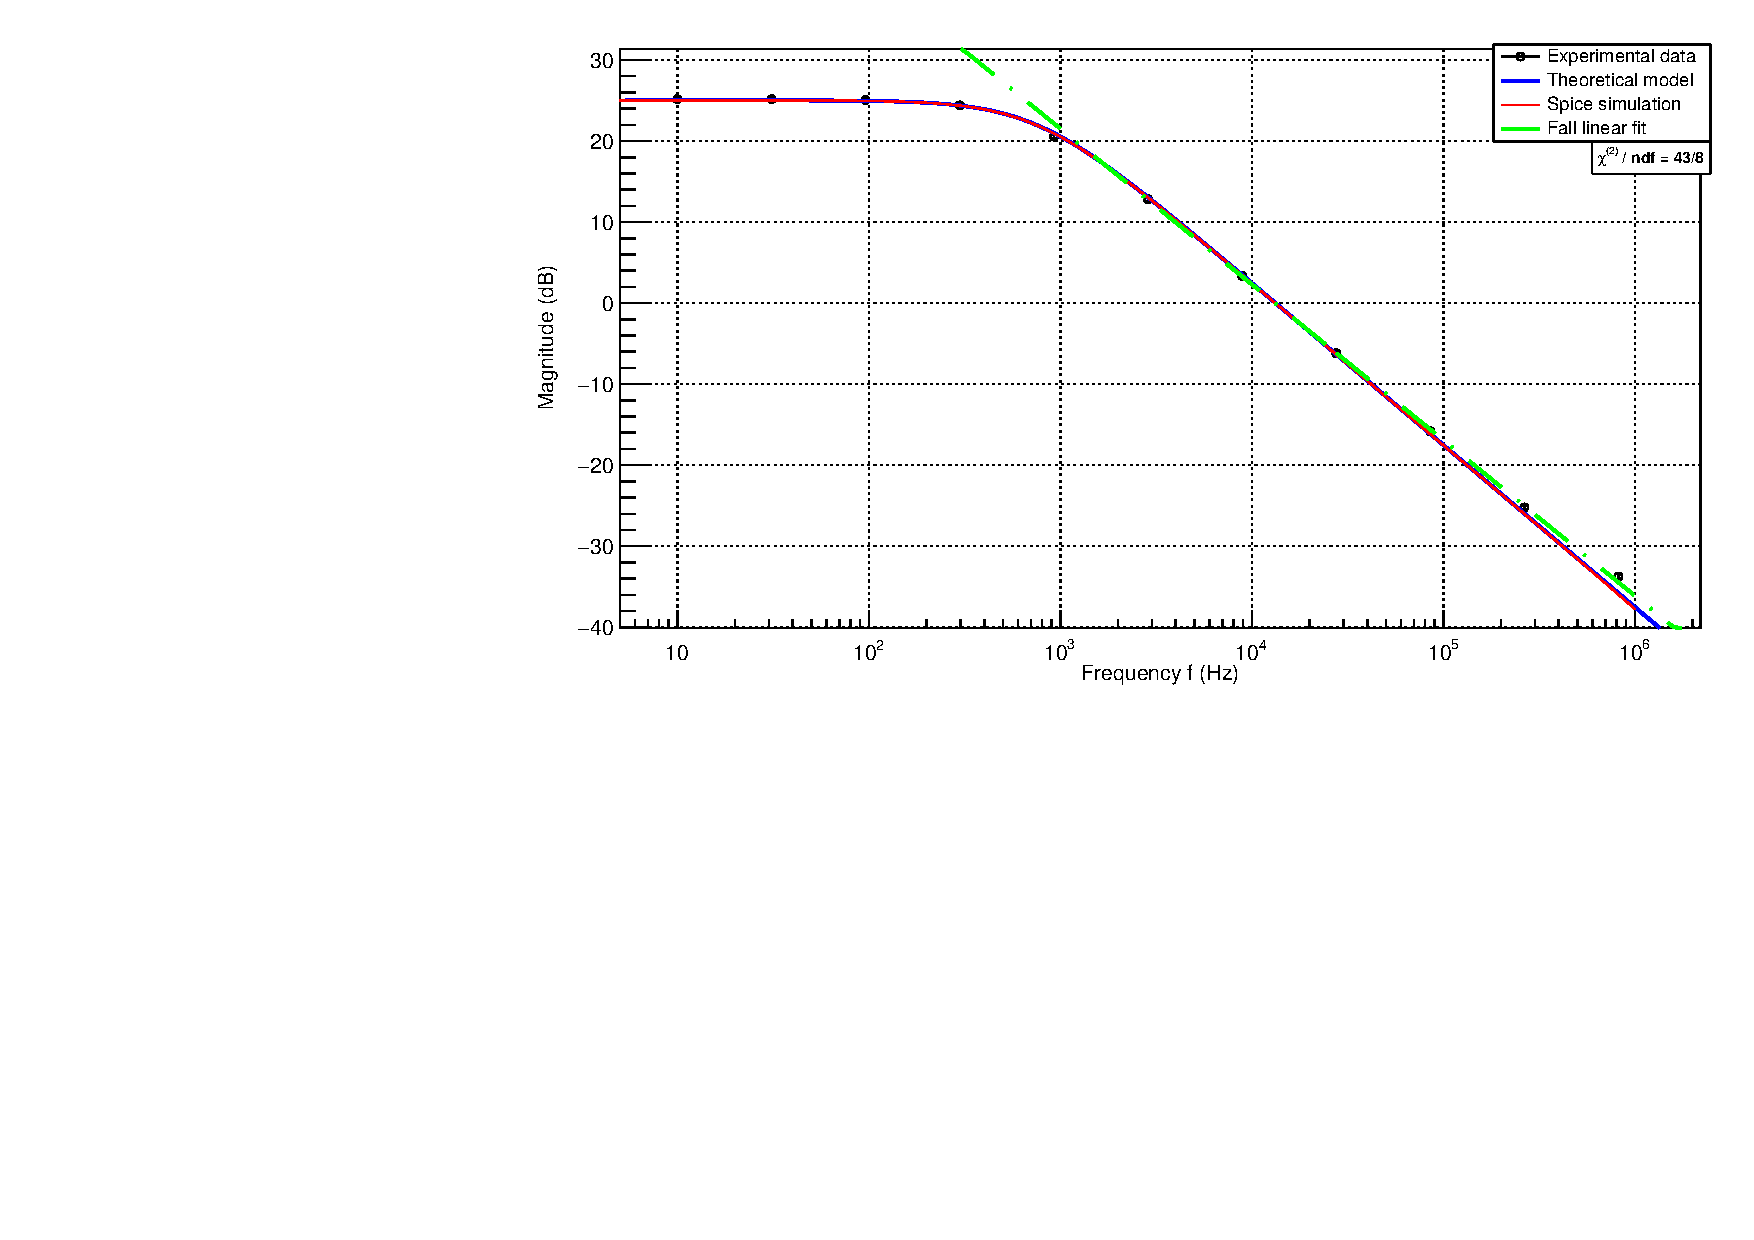
\includegraphics[scale=0.4, angle=0]{bodepreamp.pdf}
\caption{Grafico di Bode del circuito preamplificatore}
\label{fig:bodepreamp}
\end{figure}
\end{center}

<<<<<<< HEAD
\section{Circuito formatore}
\subsection{Shaper base CR-RC}
\subsubsection{Breve discussione del circuito}

Il secondo passo per la costruzione della catena elettronica consiste invece nella costruzione del circuito formatore il cui schema è riportato
in figura (\ref{fig:shaper})
\begin{center}
    \begin{figure}[H]
    \centering
    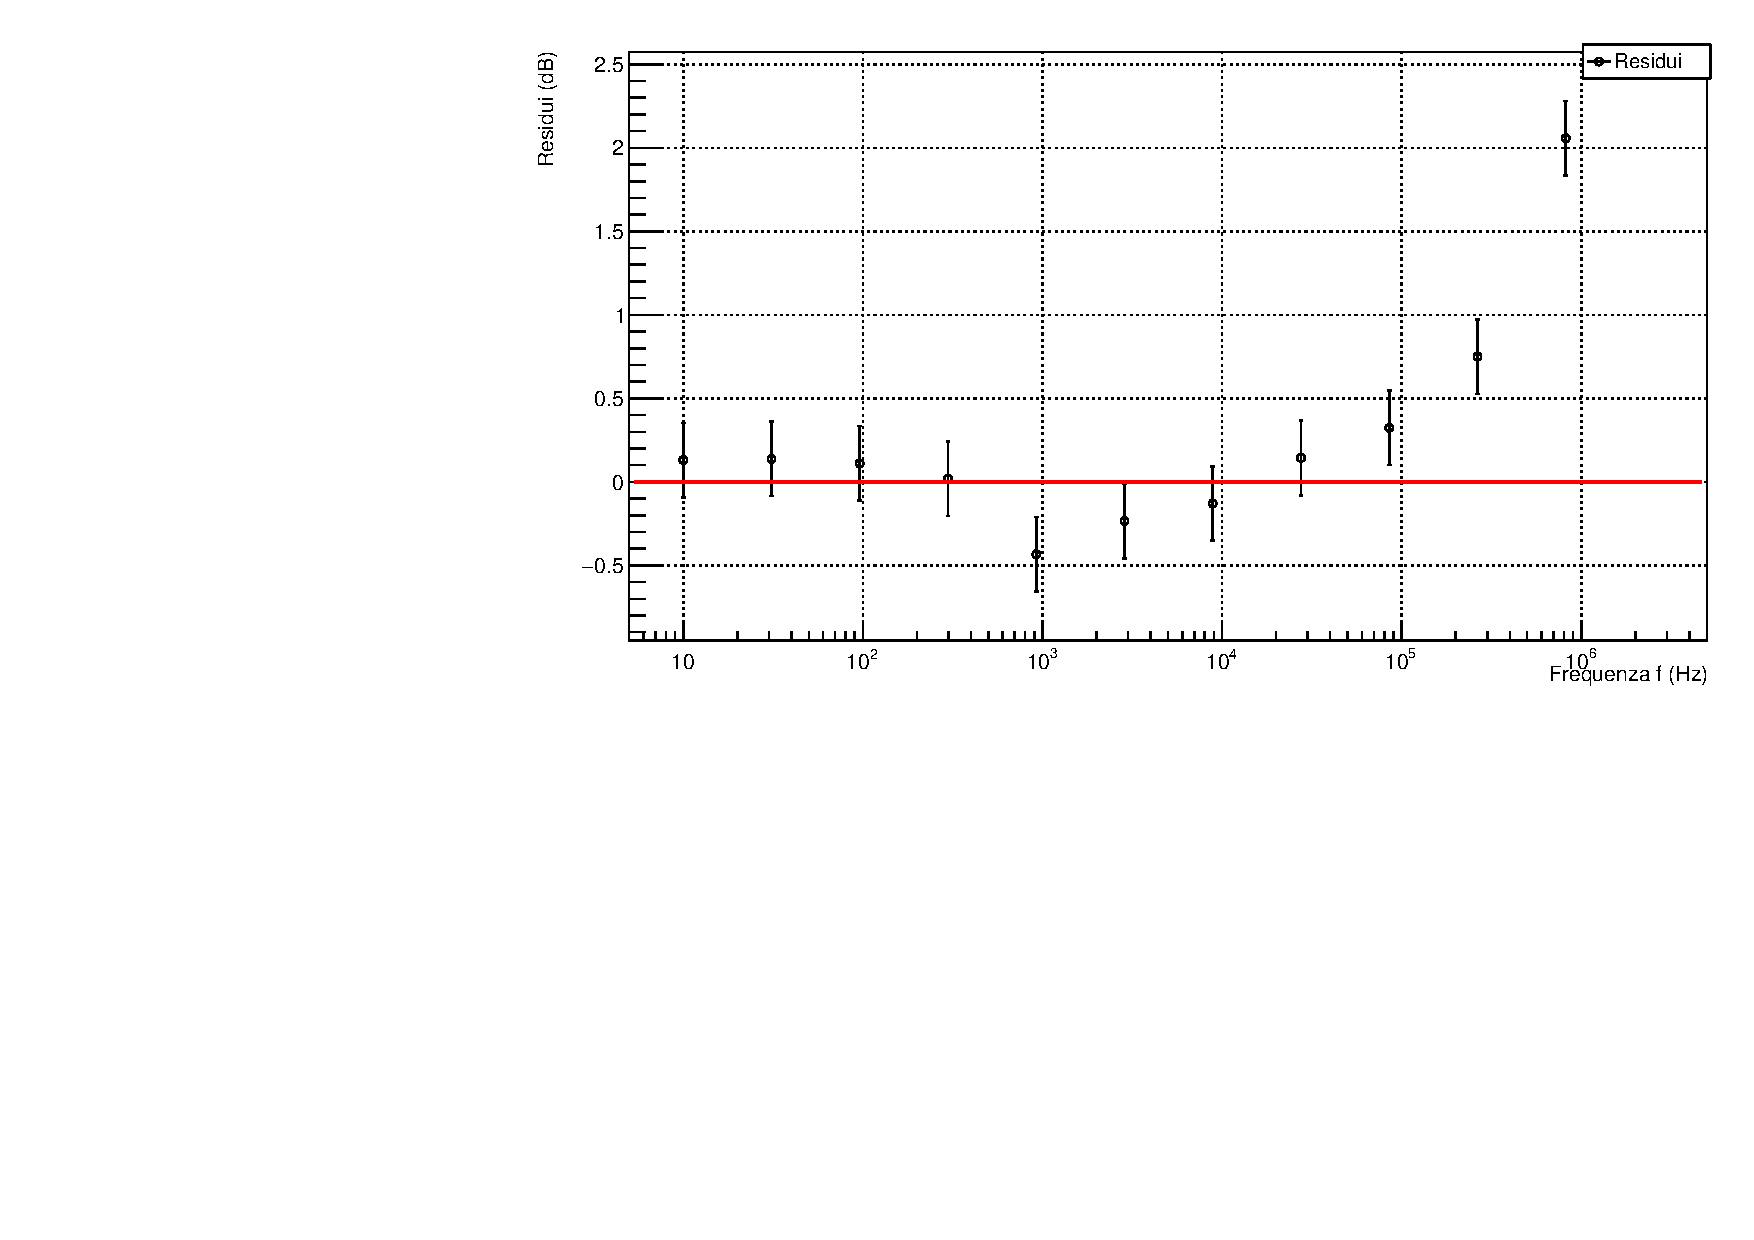
\includegraphics[scale=0.4, angle=0]{bodepreampresidui.pdf}
    \caption{Grafico del grafico di Bode}
    \label{fig:bodepreamp_res}
    \end{figure}
    \end{center}
    
    Si osserva che i dati giacciono correttamente sulla simulazione e anche il modello teorico appare adeguato, nonostante il grafico 
    dei residui mostri una certa incompatibilità delle alte frequenze. COMMENTO
\begin{center}
    \begin{figure}[H]
    \centering
    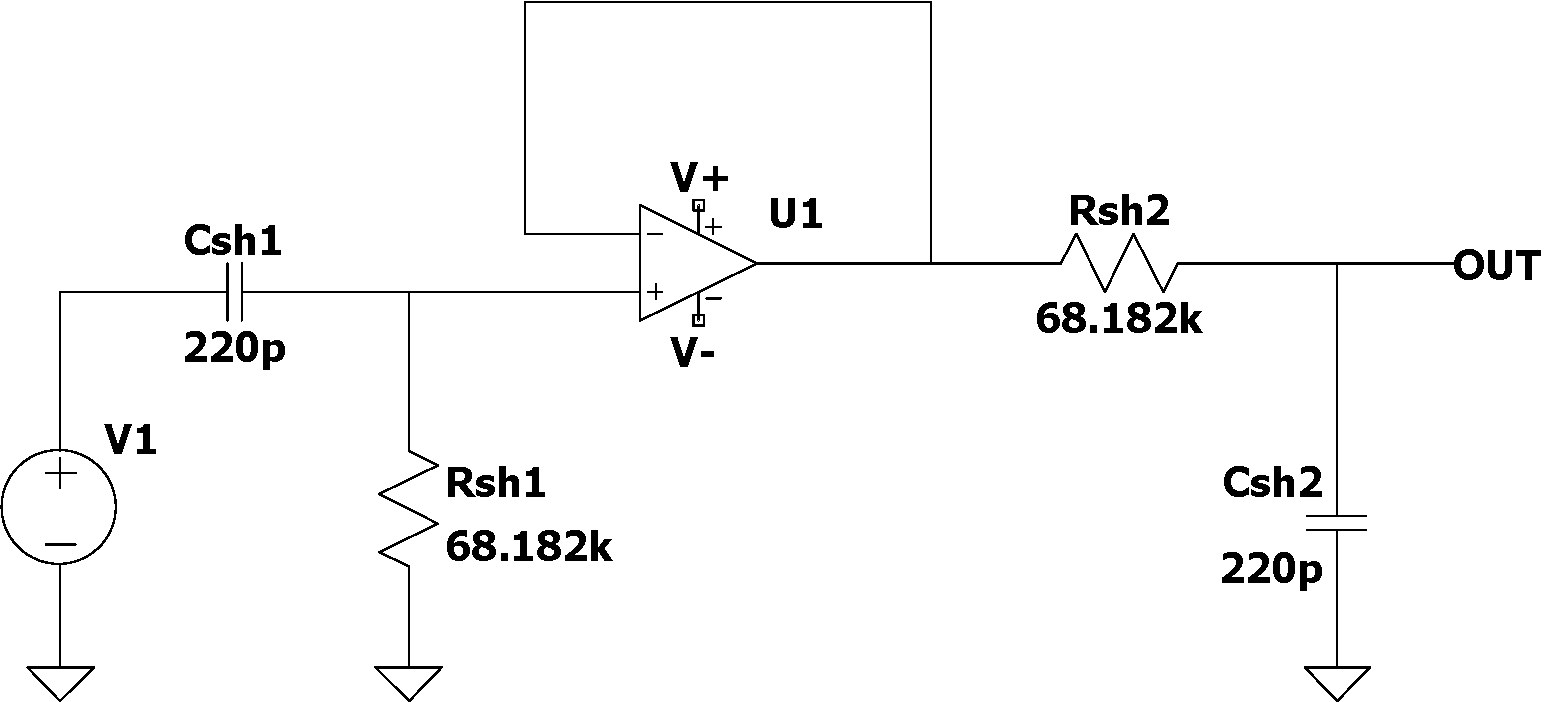
\includegraphics[scale=0.1875, angle=0]{shaper.pdf}
    \caption{Circuito formatore}
    \label{fig:shaper}
    \end{figure}
\end{center}


Per la costruzione del buffer, necessario per disaccoppiare gli stadi CR e RC si è utilizzato il secondo opamp presente nel transistor TL082.

Si specifica inoltre che i valori di $C_{sh}^{(1)}=C_{sh}^{(2)}$ e $R_{sh}^{(1)}=R_{sh}^{(2)}$ sono stati scelti in modo da ottenere il valore di $\tau_{sh}$ indicato nel logbook.

La funzione di trasferimento in funzione di $\omega$ è la seguente:
\begin{equation}
H(\omega)=\frac{\omega \tau}{1+\omega^2\tau^2}
\end{equation}

Si è quindi ottenuta la funzione $V_{out}(t)$ facendo l'antitrasformata della funzione nel dominio delle frequenze:

$$    V_{out}(t)= - \frac{V_0}{\tau} t \cdot e^{-\frac{t}{\tau}} $$

\subsubsection{discussione dei dati}
Si è nuovamente impostata sul generatore di funzioni un'onda quadra di frequenza di ?? Hz e ampiezza pari a $V_{in}^{th}$
in modo che simuli il comportamento di un preamplificatore ideale che mantenga il segnale alto per un tempo indefinito.

Sapendo che $t_{th}=R_{sh}^{(1)} C_{sh}^{(1)} = R_{sh}^{(2)} C_{sh}^{(2)}=220 \mu s$ si sono scelti e misurati i seguenti valori:
$$
R_{sh}^{(1)} = (68.305  \pm )k\Omega \quad\quad \sigma_{\%}=  \%
$$
$$
R_{sh}^{(2)} = (68.075  \pm )k\Omega \quad\quad \sigma_{\%}=  \%
$$
$$
C_{sh}^{(1)}= (234 \pm  )pF \quad\quad \sigma_{\%}=  \%
$$
$$
C_{sh}^{(2)}= (234 \pm  )pF \quad\quad \sigma_{\%}=  \%
$$

dove l'errore è stato calcolato secondo quanto scritto in appendice tenendo conto delle specifiche del multimetro Metrix 32292 relative ad un fondoscala di 
100 k$\Omega$ per le resistenze e di 1000 pF per le misure delle capacità.

Mediante i cursori si è quindi misurato il valore massimo (in valore assoluto) $V_{sh}^{max}=346 \pm mV$ e il tempo corrispondente $\tau_{sh}^{max}=15.6 \pm \mu s$, dove gli errori 
sono stati calcolati seguendo quanto scritto in appendice, si è utilizzato una divisione pari a 50 mV per l'asse verticale e pari a 25 $\mu$s per l'asse 
orizzontale.

Si è proceduto misurando un set di 10 punti della curva (riportati in in appendice), e si è ottenuto il seguente fit 
 
FIT + RESIDUI

Si è infine nuovamente studiato il comportamento del circuito al variare della frequenza (le misure sono riportate in appendice); si è ottenuto il seguente grafico di Bode

\begin{center}
    \begin{figure}[H]
    \centering
    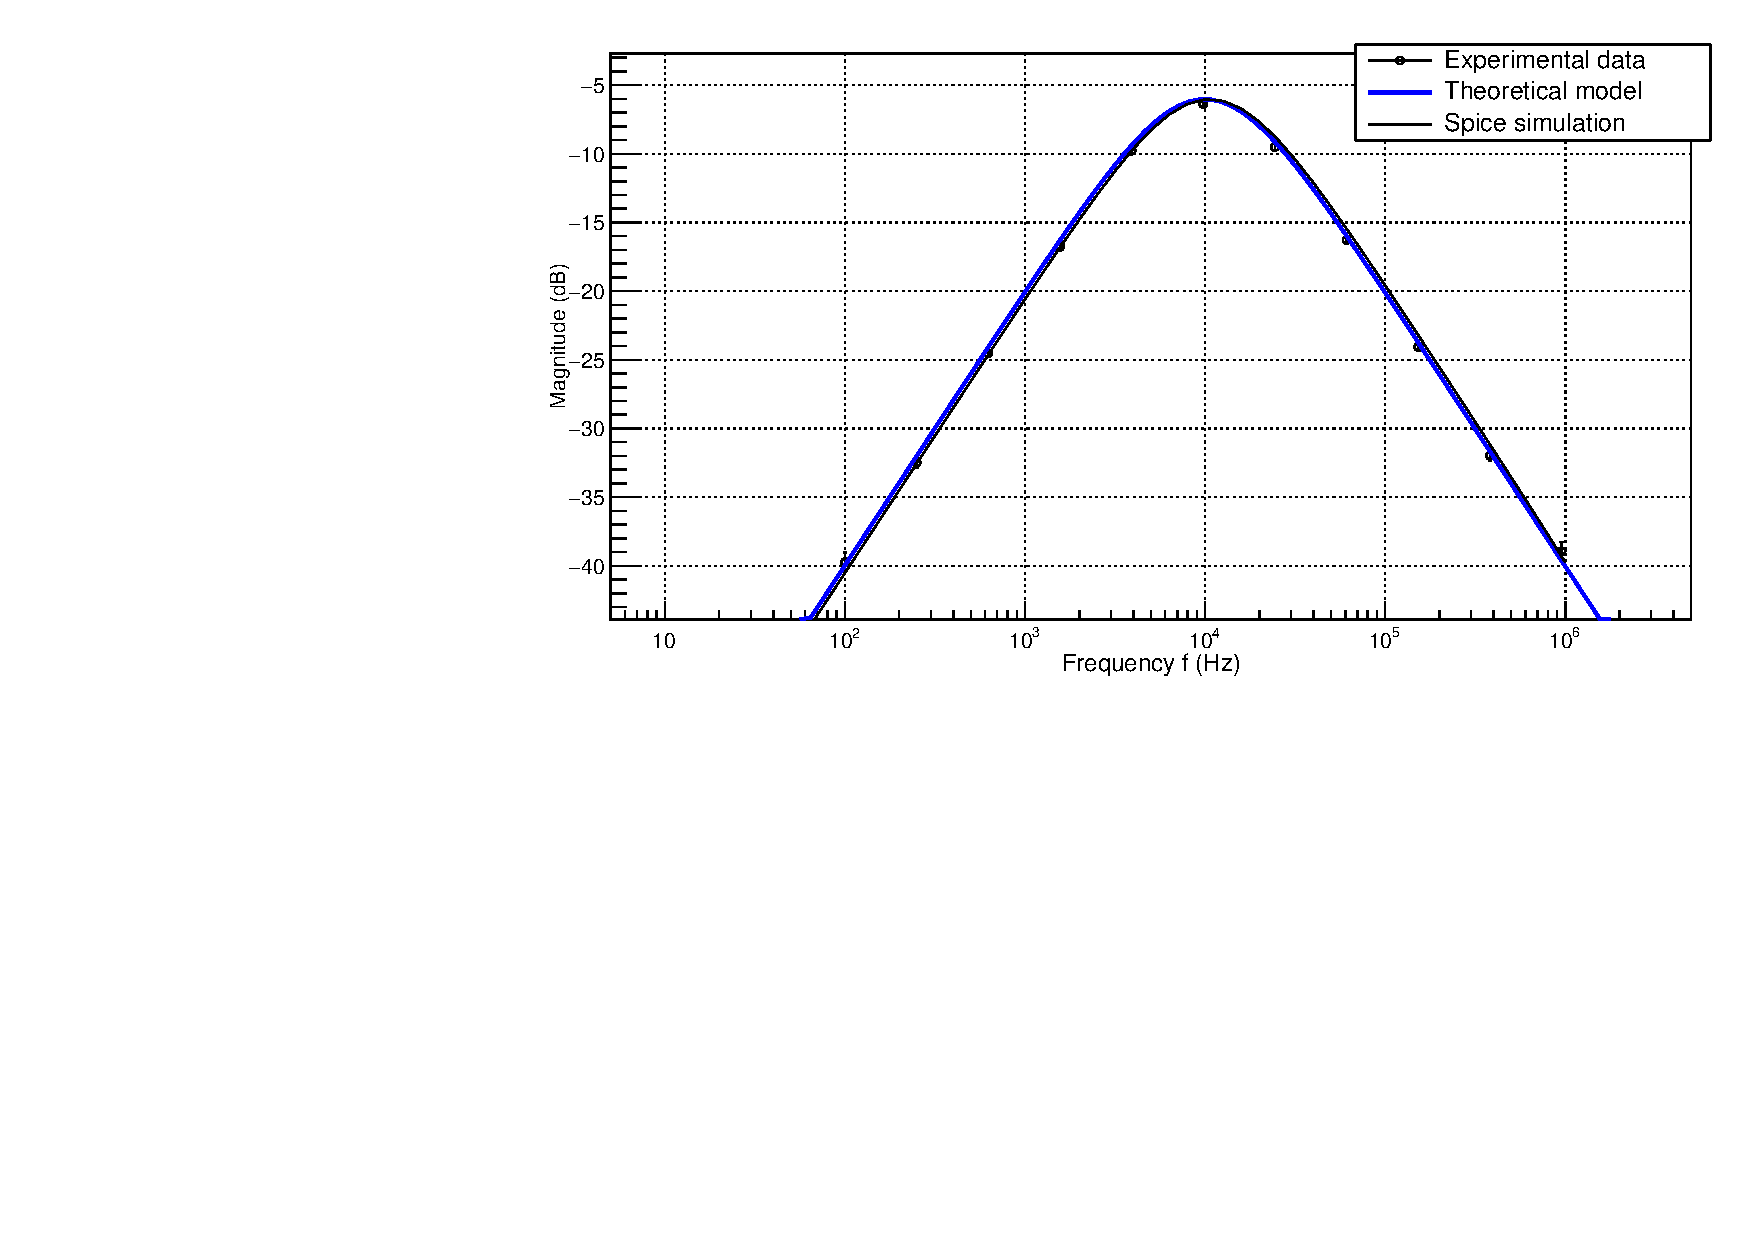
\includegraphics[scale=0.375, angle=0]{bodeshaper_no_pz.pdf}
    \caption{}
    \label{fig:bodeshaper_no_pz}
    \end{figure}
\end{center}

\begin{center}
    \begin{figure}[H]
    \centering
    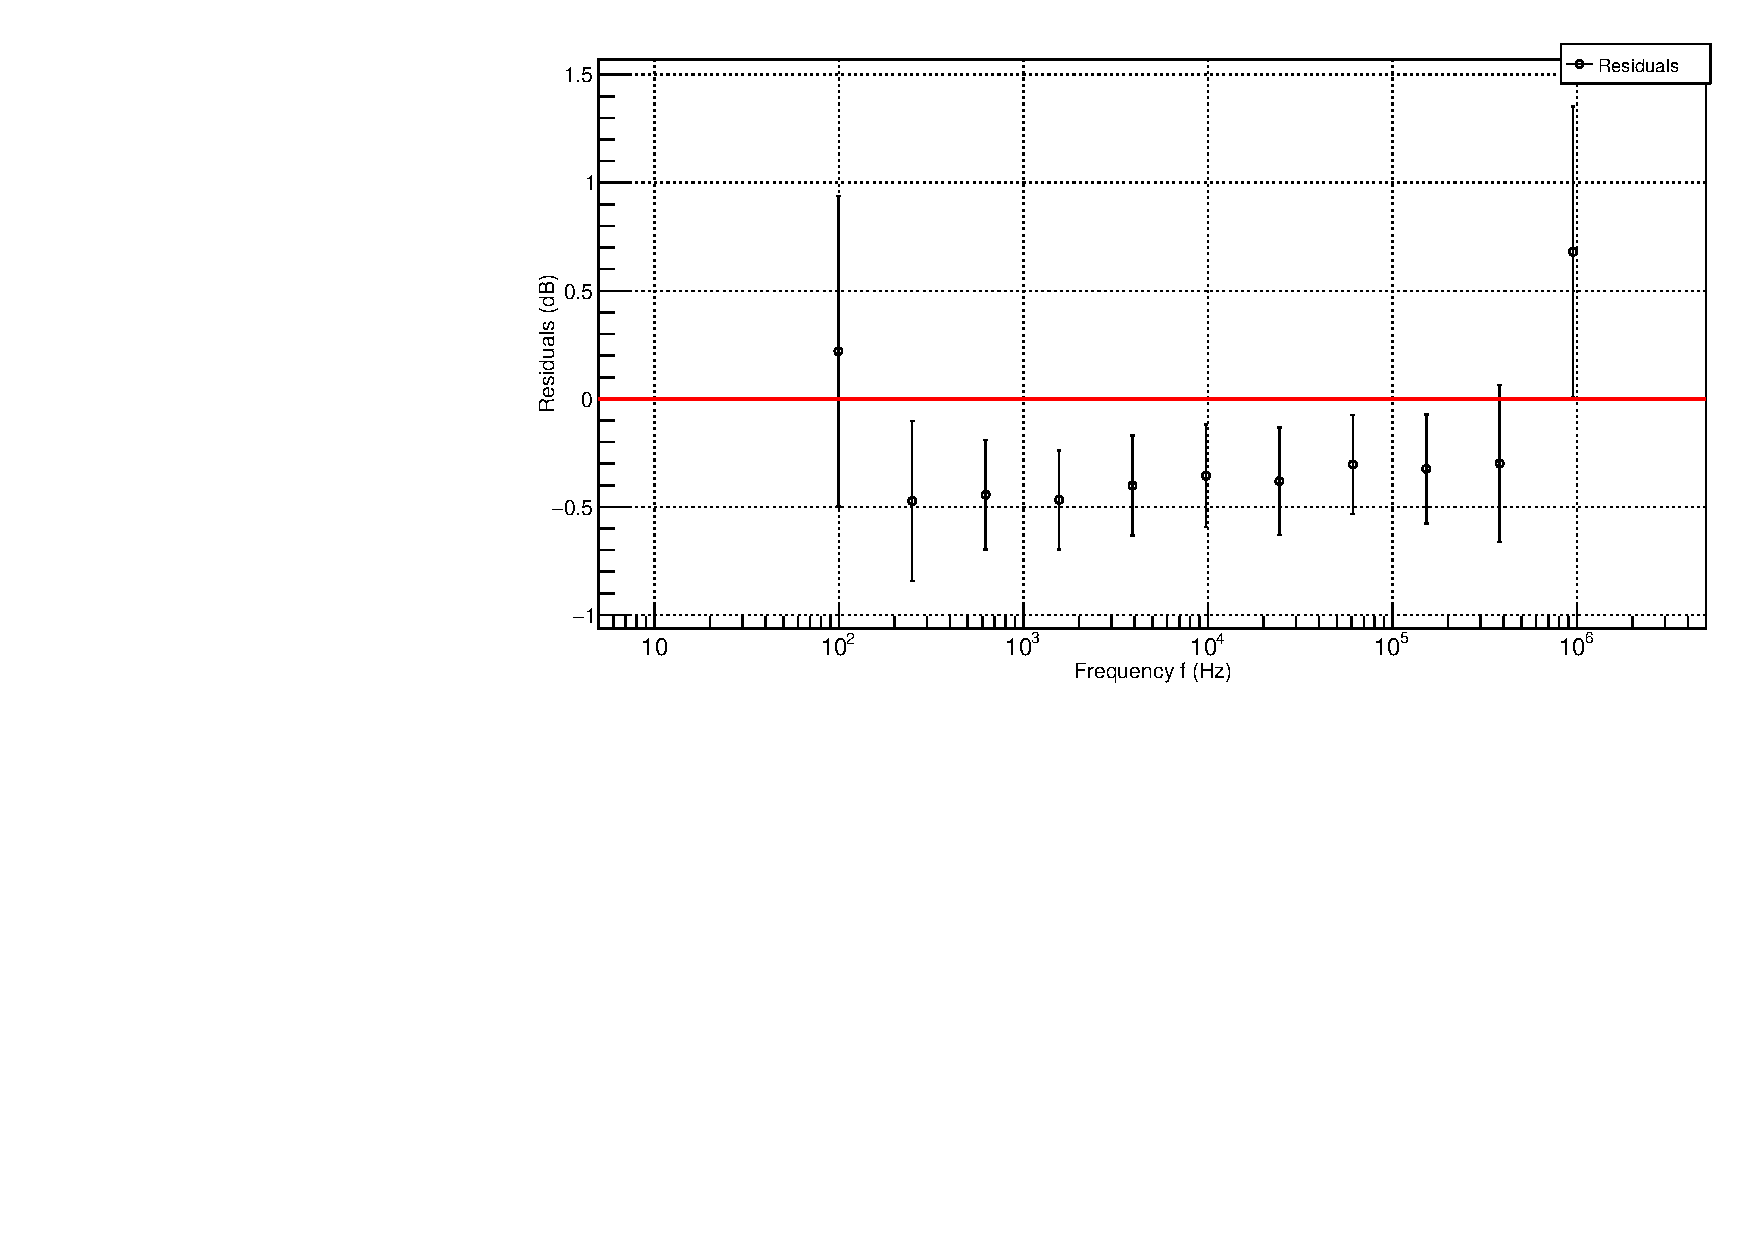
\includegraphics[scale=0.3875, angle=0]{bodeshaperresidui_no_pz.pdf}
    \caption{ }
    \label{fig:bodeshaperresidui_no_pz}
    \end{figure}
\end{center}

\subsection{Shaper compensato}
\subsubsection{Breve discussione del circuito}

\begin{center}
    \begin{figure}[H]
    \centering
    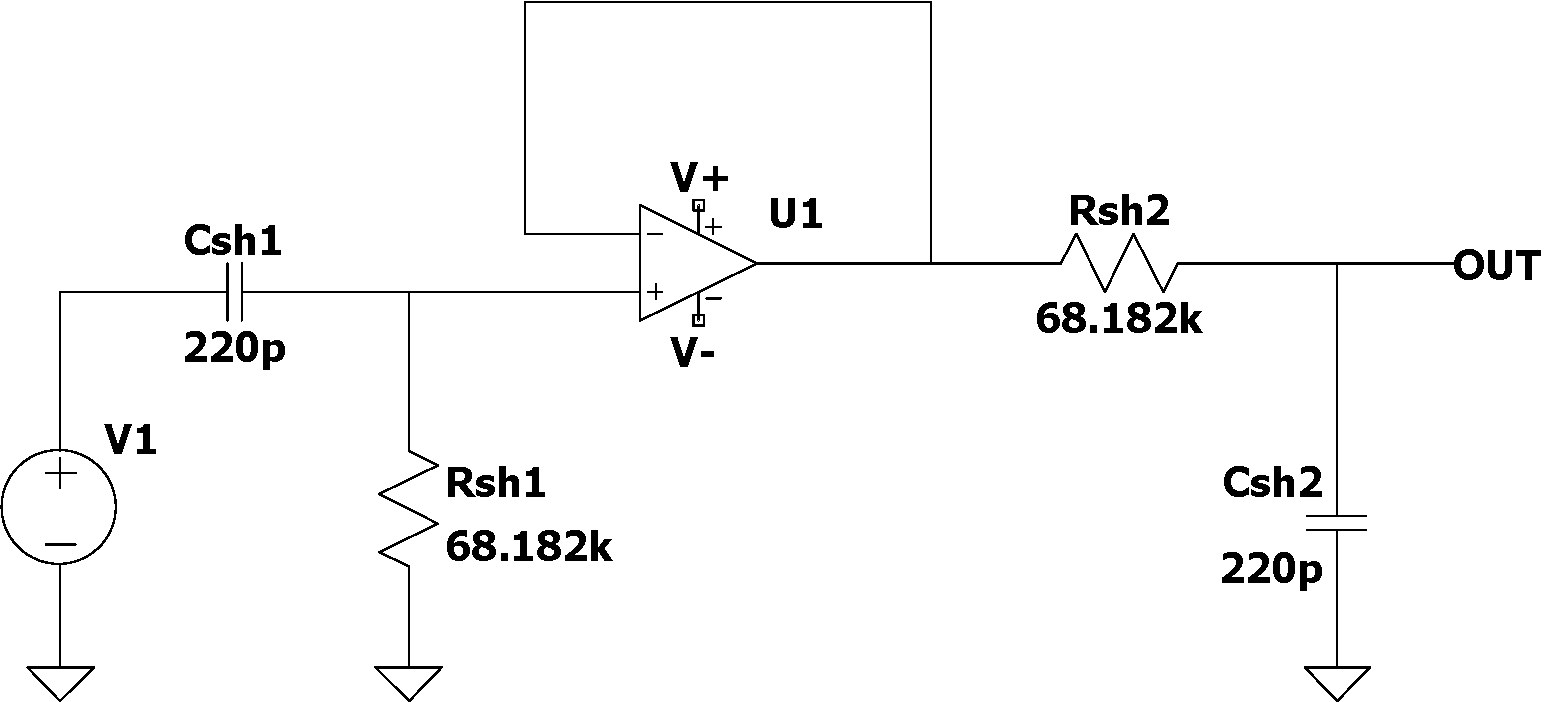
\includegraphics[scale=0.1875, angle=0]{shaper.pdf}
    \caption{Circuito formatore}
    \label{fig:shaper}
    \end{figure}
\end{center}


\subsubsection{discussione dei dati}


\begin{center}
    \begin{figure}[H]
    \centering
    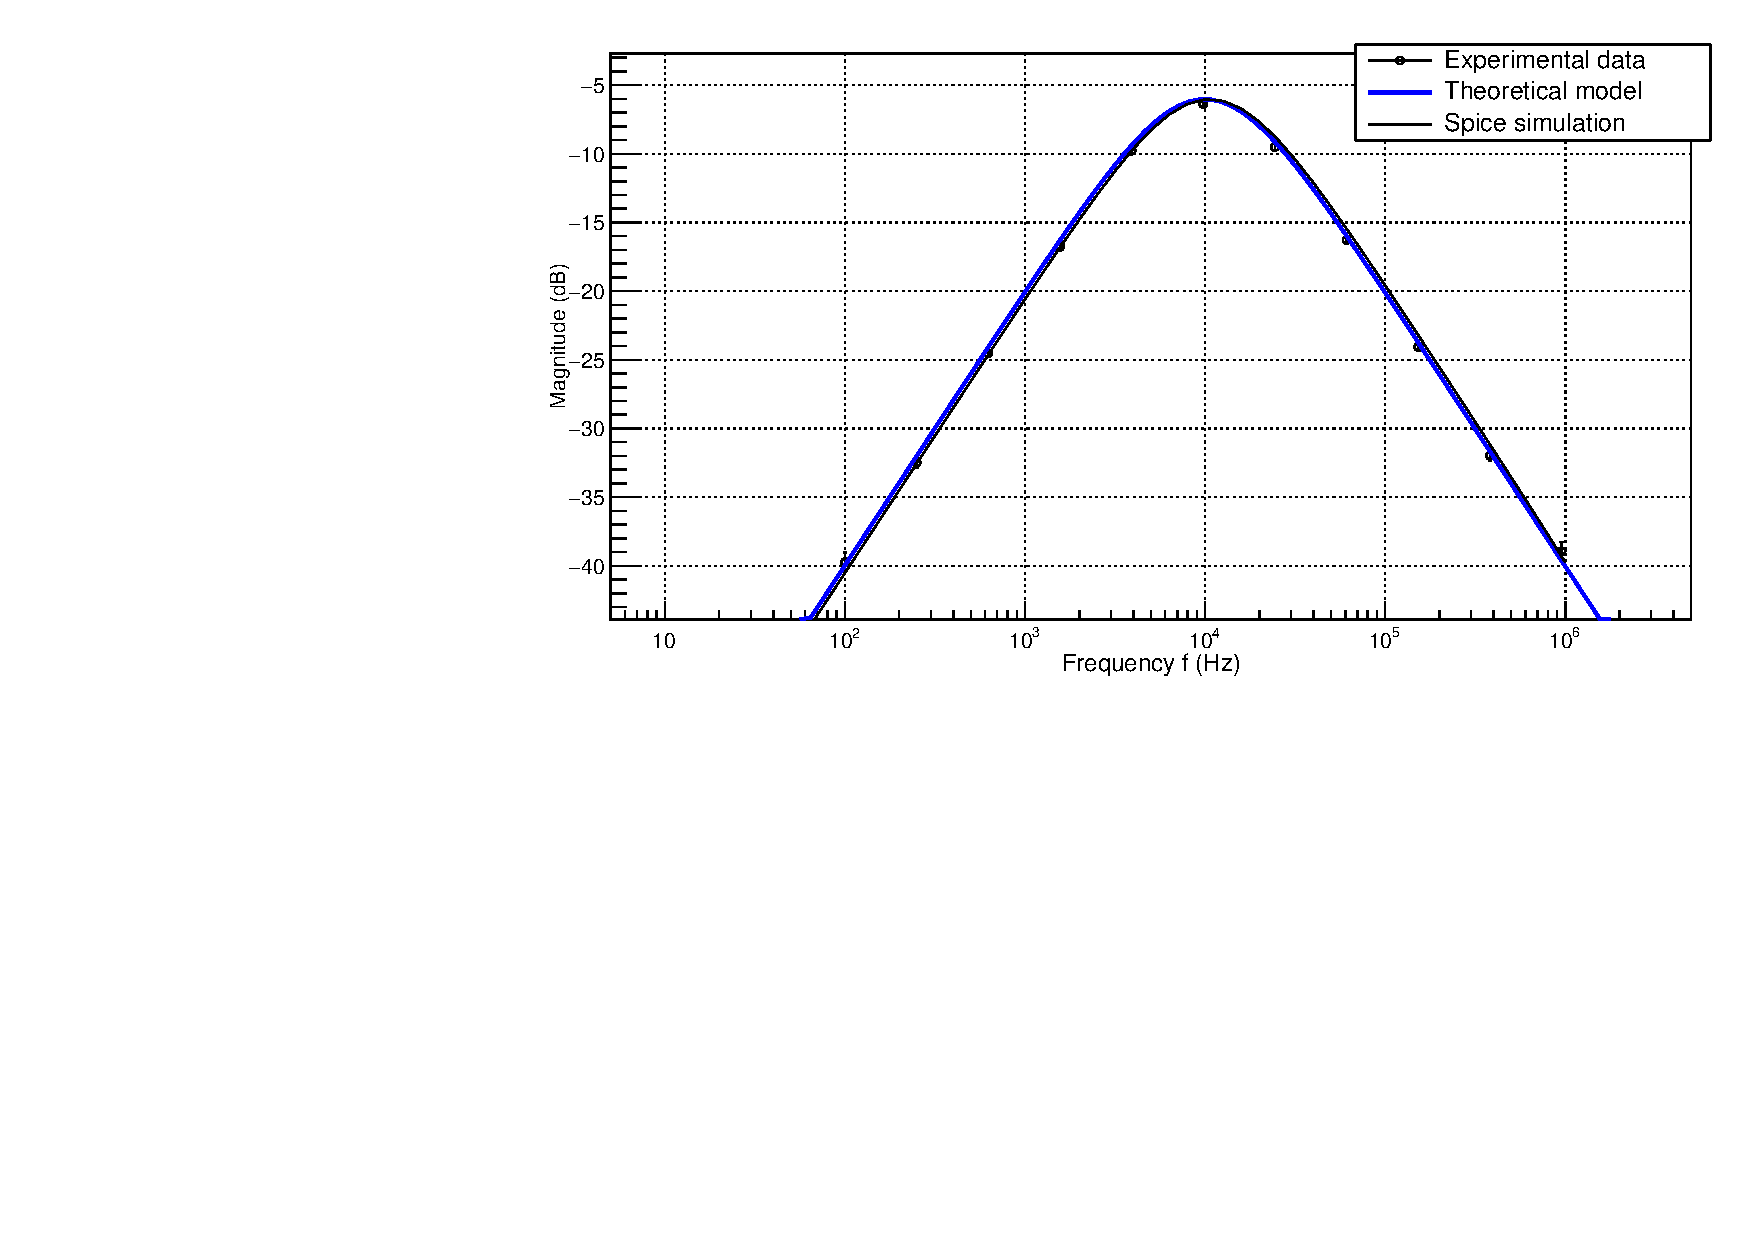
\includegraphics[scale=0.375, angle=0]{bodeshaper_no_pz.pdf}
    \caption{}
    \label{fig:bodeshaper_no_pz}
    \end{figure}
\end{center}
\section{Conclusioni}


\appendix
\section{Appendici}
\label{appendice}
\subsection{Costruzione dell'errore sulle misure}
\label{Calcerr}

Nel trattare i dati rilevati dall'oscilloscopio nel corso dell'esperienza si sono assegnati gli errori alle misure tenendo conto che ogni misura è affetta da un'incertezza di origine sistematica e da una di lettura, dovuta al posizionamento dei cursori sulla schermata. Per semplificare il calcolo degli errori, si sceglie di considerare un errore massimo $\Delta_{\%}$ di tipo percentuale per identificare il contributo sistematico presente nella presa dati, e un errore massimo $\Delta_{lett}$ per coprire le fluttuazioni casuali. La percentuale del valore letto da utilizzare come $\Delta_{\%}$ è del $3\%$ per le tensioni e dello $0.01\%$ sui tempi: per quanto riguarda invece l'errore di lettura, si è considerato 1/10 della divisione utilizzata.
Tuttavia, poiché l'errore percentuale sui tempi è sempre decisamente trascurabile rispetto a quello di lettura, lo si è omesso nel calcolo dell'incertezza totale.

Infine, si precisa che tutti i risultati sono presentati con un errore non massimo, ma di tipo statistico: si riporta la regola di conversione, in ipotesi di distribuzione uniforme per l'errore sistematico e in ipotesi di distribuzione triangolare per l'errore di lettura.

\begin{equation}
\sigma_{\%}=\frac{2\Delta_{\%}}{\sqrt{12}} \quad \quad \sigma_{lett}=\frac{2\Delta_{lett}}{\sqrt{24}}
\end{equation}

Un meccanismo analogo vale per le misure dirette di grandezze quali resistenze e capacità effettuate con il multimetro: anche in questo caso abbiamo un contributo sistematico e uno casuale, il primo dato ancora da un errore percentuale e il secondo da un errore in digit. Tale contributo in digit è dato da $\Delta_{dgt}=ns$ dove $n=\#digit$ è un numero intero riportato sul manuale dello strumento e $s$ è la sensibilità usata nella lettura del valore. Anche qui si utilizza la conversione in errori statistici in ipotesi di distribuzione uniforme.

\subsection{Commento sull'accettazione/rifiuto dei fit}
Nel corso della relazione sono stati riportati diverse volte i parametri per la verifica della bontà del fit, sostenendo che essi permettessero di accettare o rifiutare l'interpolazione.


Per quanto riguarda i valori di $\chi^{(2)}$, l'ipotesi che il fit descriva i dati viene accettata o rifiutata con 0.90 CL, mentre
per il valore di $t$ di Student l'ipotesi di non correlazione è stata rifiutata o accettata con lo stesso CL.


\subsection{Tabella delle compatibilità}
\medskip
\begin{table}[H]
    \centering
    \begin{tabular}{c}
        %\hline
        \begin{Large}
        $\lambda=\frac{|a-b|}{\sqrt{\sigma_a^2+\sigma_b^2}}$
        \end{Large}\\
        %\hline
    \end{tabular}
    \hspace{0.5cm}
    \begin{tabular}{cc}
        \toprule
        &       \textbf{Compatibilità   }       \\
        \midrule
        0$\leq \lambda$<1   &Ottima                 \\
        1<$\leq \lambda$<2   &Buona                  \\
        2<$\leq \lambda$<3   &Accettabile            \\
        3<$\leq\lambda$<5   &Pessima                \\
        $ \lambda \geq $  5     &Non compatibile        \\
        \bottomrule
    \end{tabular}
    \caption{Indicazioni lettura compatibilità}
\end{table}

\subsection{Dati sperimentali}
\end{document}
